\documentclass{article}

\usepackage{swiftnav}


\usepackage{draftwatermark}
\SetWatermarkLightness{0.9}
\SetWatermarkText{Preliminary}
\SetWatermarkScale{1}

% Suppress numbers from section headings (but preserve PDF TOC).
\makeatletter
\renewcommand\@seccntformat[1]{}
\makeatother

\newenvironment{mpar}{\par\noindent\minipage{\linewidth}}{\endminipage\par}
%\setlength{\skip\mpfootins}{2cm}
\renewcommand{\thempfootnote}{(\arabic{mpfootnote})}

% ---------------------------------------------------------------------------
\usepackage[section]{placeins}
\version{2.3.1}
\title{Piksi for UAV Aerial surveying}
\mysubtitle{RTK direct georeferencing with Swift Navigation's Piksi GPS receiver}
\author{Dennis Zollo, Rai Gohalwar}
\date{\today}

\begin{document}

\maketitle

\thispagestyle{firstpage}

\section{Abstract}
\label{sec:abstract}
This whitepaper presents using Piksi, a Carrier Phase differential GPS sensor, to georeference aerial images from an unmanned aerial vehicle (UAV) for surveying use cases.
It presents both the integration and flight planning methods as well as the surveying  results from flight data as processed by the PIX4D photogrammetry software.
Lastly, the value proposition of using RTK GPS for aerial surveying is evaluated.
\tableofcontents
\newpage
\section{Overview}
\label{sec:Overview}
This is the overview
\section{Equipment and Setup}
\label{sec:equipment}
Camera, focal length, quadcopter
Radios
\section{Method}
\label{sec:method}
Site selection
GCP surveying (skylark)
Mission Planning (mission planner)
Camera setup (exposure, etc)
\section{Post-Processing Techniques}
\begin{figure}
\begin{center}
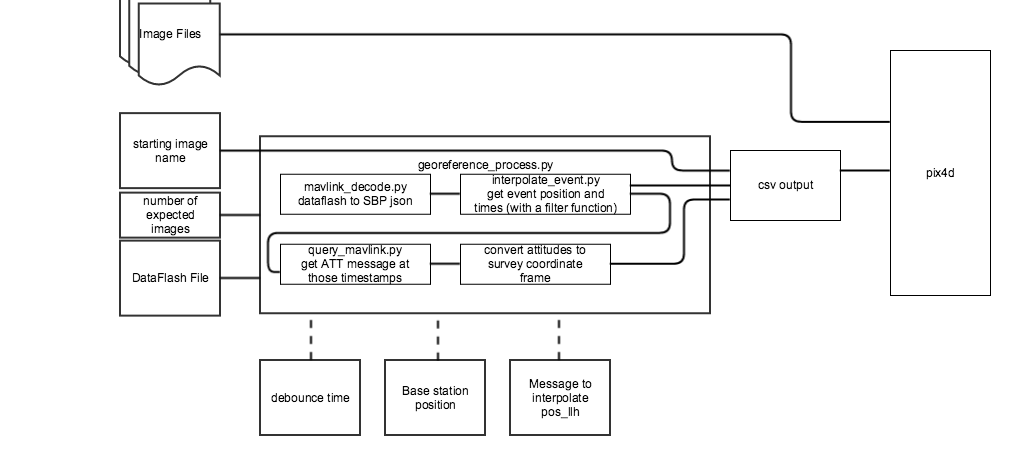
\includegraphics[width=7in]{images/uav_survey_processing_architecture.png}
\end{center}
\end{figure}
\begin{tabular}[pos]{l|l|l|l|l}
Label & Description & Notes & GPS Sensor & GCP
\end{tabular}
\thispagestyle{lastpage}
\end{document}
